% Лекц 16. Өргөтгөсөн тодорхой интеграл
% Эх: latex/lectures/lec16-improper-integral.tex (scripts/latex_to_beamer.py-ээр хөрвүүлсэн)
% Frame бүр слайдад нэг (эсвэл allowframebreaks-аар хэд хэдэн) хуудас болно;
% хэвлэх хувилбарт frame-ийн хил харагдахгүй, текст үргэлжилсэн байна.

\MathLecture{16}{Өргөтгөсөн тодорхой интеграл}

\begin{frame}[allowframebreaks]{Өргөтгөсөн тодорхой интеграл}
Тодорхой интегралын дээд эсвэл доод хил нь $\infty$ (эсвэл $-\infty$) байх, эсвэл 
интегралчлах функц нь интегралчлах мужын зарим цэг дээр тасралттай байх 
тохиолдолд интегралыг нийлбэрийн хязгаараар тодорхойлох боломжгүй юм. 
Ийм интегралуудыг бодох шаардлага гардаг тул эдгээр интегралыг хязгаар ашиглан тодорхойлдог.
\end{frame}

\section{Зааглагдаагүй мужаар авсан интеграл}
\begin{frame}[allowframebreaks]{Зааглагдаагүй мужаар авсан интеграл}
\begin{definition}[I төрлийн өргөтгөсөн интеграл]
$f$ функц нь $[a,+\infty)$ дээр тодорхой байг. Хэрэв
\[
\lim_{t\to\infty}\int_a^{t} f(x)\,dx
\]
хязгаар оршин байвал түүнийг $f(x)$ функцээс $[a,\infty)$ завсараар авсан тодорхой интеграл гэнэ.  

\[
\int_a^{\infty} f(x)\,dx := \lim_{t\to\infty}\int_a^{t}f(x)\,dx.
\]

Хэрэв хязгаар төгсгөлөг утгатай байвал интегралыг \textbf{нийлдэг}, бусад үед \textbf{сарнидаг интеграл} гэнэ.
\end{definition}

Доод хил эсвэл хоёр хил нь зааглагдаагүй үед адилаар тодорхойлно.

\[
\int_{-\infty}^{b} f(x)\,dx := \lim_{t\to -\infty}\int_t^{b}f(x)\,dx,
\qquad
\int_{-\infty}^{\infty} f(x)\,dx := 
\int_{-\infty}^{c} f(x)\,dx + \int_{c}^{\infty} f(x)\,dx.
\]
\end{frame}

\begin{frame}[allowframebreaks]{Зааглагдаагүй мужаар авсан интеграл}
\begin{example}\label{x^{-2}}
$y=\dfrac{1}{x^2}$ ($x\ge1$) графикийн доорх талбайг олъё:
\[
\int_{1}^{\infty} \frac{dx}{x^2}
= \lim_{t\to\infty}\int_{1}^{t} x^{-2}\,dx
= \lim_{t\to\infty}\left[-x^{-1}\right]_{1}^{t}
= \lim_{t\to\infty}\left( -\frac{1}{t} + 1\right)
= 1.
\]
Иймээс
\[
\int_{1}^{\infty}\frac{dx}{x^2} = 1 \quad (\text{нийлнэ}).
\]
\end{example}
\end{frame}

\section{Үл зааглагдах функцийн интеграл}
\begin{frame}[allowframebreaks]{Үл зааглагдах функцийн интеграл}
\begin{definition}[II төрлийн өргөтгөсөн интеграл]
$f$ функц нь $(a,b)$ дээр тасралтгүй тодорхойлогдсон боловч $x=a$ дээр төгсгөлгүй тасралттай байг.  
Хэрэв
\[
\lim_{t\to a+}\int_{t}^{b} f(x)\,dx
\]
хязгаар оршин байвал түүнийг $y=f(x)$ функцээс $(a,b)$ завсараар авсан тодорхой интеграл гэнэ.
\[
\int_{a}^{b} f(x)\,dx := \lim_{t\to a+}\int_{t}^{b}f(x)\,dx.
\]
Хэрэв $x=b$ дээр төгсгөлгүй тасралттай бол
\[
\int_a^{b}f(x)\,dx = \lim_{t\to b-}\int_{a}^{t} f(x)\,dx.
\]
Хэрэв хязгаар төгсгөлөг байвал интегралыг \textbf{нийлдэг}, үгүй бол \textbf{сарнидаг интеграл} гэнэ.
\end{definition}
\end{frame}

\begin{frame}[allowframebreaks]{Үл зааглагдах функцийн интеграл}
\begin{example}\label{x^{-1/2}}
$f(x) = \dfrac{1}{\sqrt{x}}$ нь $(0,1)$ дээр тодорхойлогдох боловч $x\to 0^{+}$ үед $f(x)\to\infty$.
Иймд 
\[
\int_{0}^{1}\frac{dx}{\sqrt{x}}
= \lim_{t\to0+}\int_{t}^{1} x^{-1/2}\,dx
= \lim_{t\to0+}\left[2\sqrt{x}\right]_{t}^{1}
= \lim_{t\to0+}(2 - 2\sqrt{t})
= 2.
\]
Иймээс интеграл \textbf{нийлнэ}.
\end{example}
\end{frame}

\begin{frame}[allowframebreaks]{Үл зааглагдах функцийн интеграл}
\begin{example}\label{x^-1}
\[
\int_{0}^{1}\frac{dx}{x}
= \lim_{t\to0+}\int_{t}^{1} \frac{dx}{x}
= \lim_{t\to0+} [\ln x]_{t}^{1}
= \lim_{t\to0+}(0 - \ln t)
= +\infty.
\]
Иймээс интеграл \textbf{сарнина}.
\end{example}
\end{frame}

\section{Нийлэлт, сарнилтыг тодорхойлох шинжүүр}
\begin{frame}[allowframebreaks]{Нийлэлт, сарнилтыг тодорхойлох шинжүүр}
\begin{theorem}Жиших шинжүүр]
$x\ge a$ үед $0\le f(x)\le g(x)$ байг.

\begin{enumerate}
\item Хэрэв $\displaystyle\int_{a}^{\infty} g(x)\,dx$ нийлбэл  
\quad $\displaystyle\int_{a}^{\infty} f(x)\,dx$ мөн нийлнэ.
\item Хэрэв $\displaystyle\int_{a}^{\infty} f(x)\,dx$ сарнивал  
\quad $\displaystyle\int_{a}^{\infty} g(x)\,dx$ мөн сарнина.
\end{enumerate}
\end{theorem}
Харьцуулах шинжүүр хэрэглэхийн тулд өгсөн интегралтай төстэй нийлэх сарнихыг нь мэддэг интеграл авч үзэх хэрэгтэй. Ийм зорилгоор ихэвчлэн $f(x)=x^{-p}$ функцийн интегралыг авч үздэг.
\end{frame}

\begin{frame}[allowframebreaks]{Нийлэлт, сарнилтыг тодорхойлох шинжүүр}
\begin{example}[ $x^{-p}$ функцийн интеграл]
 Жишээ \ref{x^{-2}} харахад $\displaystyle\int\limits_1^{\infty}x^{-p}dx$ интеграл $p=2$ үед нийлж байна. Ерөнхий тохиолдолд дараах нөхцөл биелнэ.
 \[
\int_{1}^{\infty} \frac{dx}{x^{p}}
\quad\text{нийлэх } \Longleftrightarrow\; p>1.
\]
Тодруулбал,
\[
\int_{1}^{\infty} x^{-p}\,dx =
\begin{cases}
\displaystyle \frac{1}{p-1}, & p>1,\\[4pt]
+\infty, & p\le1.
\end{cases}
\] байна. \\
Мөн Жишээ \ref{x^{-1/2}} ба  \ref{x^-1}  харахад $\displaystyle\int\limits_1^{\infty}x^{-p} dx$ интеграл $p= 1/2$ үед нийлж, $p=1$ үед сарниж байна. Ерөнхий тохиолдолд дараах нөхцөл биелнэ.
 \[
\int_{0}^{1} x^{-p}\,dx
\quad\text{нийлэх } \Longleftrightarrow\; p<1.
\]

Тодруулбал,
\[
\int_{0}^{1} x^{-p}\,dx =
\begin{cases}
\displaystyle \frac{1}{1-p}, & p<1,\\[4pt]
+\infty, & p\ge1.
\end{cases}
\]
\end{example}
\end{frame}

\begin{frame}[allowframebreaks]{Нийлэлт, сарнилтыг тодорхойлох шинжүүр}
\begin{example}[Жиших шинжүүр хэрэглэх]
Дараах интеграл нийлэх эсэхийгтодорхойлоё.
\[
\int_{1}^{\infty} \frac{dx}{1+x^{3}}.
\]

Их $x$ үед $1+x^3\sim x^{3}$.
\[
0 < \frac{1}{1+x^{3}} \le \frac{1}{x^{3}}, \qquad x\ge1.
\]
жиших шинжүүрээр $p=3>1$ тул  
\[
\int_{1}^{\infty}\frac{dx}{x^{3}}
\text{ нийлэх тул}
\quad\Rightarrow\quad
\int_{1}^{\infty}\frac{dx}{1+x^{3}}
\text{ мөн нийлнэ.}
\]
\end{example}
\end{frame}

\section{Тодорхой интегралын хэрэглээ}
\subsection{Хоёр муруйн хоорондох талбай}
\begin{frame}[allowframebreaks]{Хоёр муруйн хоорондох талбай}
$y=f(x) , \, y=g(x)$ функцүүдийн графикуудын хоорондох хашигдсан $x=a , \, x=b$ хэсгийн талбайг
\[
A=\int_{a}^{b} |f(x)-g(x)|\,dx.
\]
томьёогоор олно.
\end{frame}

\begin{frame}[allowframebreaks]{Хоёр муруйн хоорондох талбай}
\begin{example} $y=2x$, $y=x^2$ муруйн хоорондох талбай ол.\\
\begin{minipage}{0.6\textwidth}
\begin{fitbox}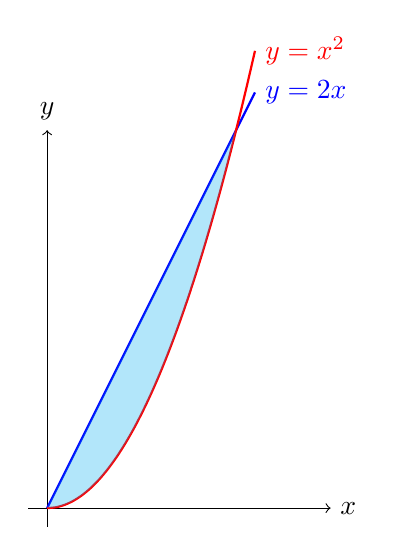
\begin{tikzpicture}[scale=1.2]
\draw[->] (-0.2,0) -- (3,0) node[right] {$x$};
\draw[->] (0,-0.2) -- (0,4) node[above] {$y$};

\draw[domain=0:2.2, smooth, variable=\x, blue, thick]
  plot ({\x},{2*\x}) node[right] {$y=2x$};

\draw[domain=0:2.2, smooth, variable=\x, red, thick]
  plot ({\x},{\x*\x}) node[right] {$y=x^2$};

\begin{scope}
\clip (0,0) --
  plot[domain=0:2] ({\x},{2*\x}) --
  plot[domain=2:0] ({\x},{\x*\x}) -- cycle;

\fill[cyan, opacity=.3] (0,0) rectangle (3,4);
\end{scope}
\end{tikzpicture}\end{fitbox}  
\end{minipage}
\begin{minipage}{0.4\textwidth}
   $y=2x$, $y=x^2$ муруйн хоорондох талбайг олохын тулд тэдгээрийн огтлолцлын цэгүүдийг олох хэрэгтэй. $2x=x^2$ тэгшитгэл бодвол $x=0,\, x=2$ шийдүүд гарна. Иймд олох талбай нь 
\[
A=\int_{0}^{2} |2x-x^2|\,dx=\int_{0}^{2} (2x-x^2)\,dx=\frac{4}{3}.
\] болно. 
\end{minipage}
\end{example}
\end{frame}

\begin{frame}[allowframebreaks]{Хоёр муруйн хоорондох талбай}
\begin{example}
    $f(x)=\cos x$, $g(x)=\sin x$, $[\pi/6,\pi/4]$ интервал дээрх талбай ол.\\
Харгалзах график зурж харвал:

\begin{center}
\begin{fitbox}\begin{tikzpicture}[scale=2]
% Axes
\draw[->] (-0.2,0)--(1.2,0) node[right]{$x$};
\draw[->] (0,-0.2)--(0,1.2) node[above]{$y$};

% Functions
\draw[domain=0:0.9,samples=100,thick,blue]
  plot(\x,{cos(\x r)}) node[right]{$y=\cos x$};

\draw[domain=0:0.9,samples=100,thick,red]
  plot(\x,{sin(\x r)}) node[right]{$y=\sin x$};

% Fill area
\fill[green!60,opacity=0.7]
  plot[domain=0.5:0.785] (\x,{cos(\x r)})
  -- plot[domain=0.785:0.5] (\x,{sin(\x r)})
  -- cycle;
\draw[dashed] (0.785,0)--(0.785,0.71);
\draw[dashed] (0.5,0)--(0.5,0.855);
\node at (0.785,-0.2) {$\tfrac{\pi}{4}$};
\node at (0.5,-0.2){$\tfrac{\pi}{6}$};
\end{tikzpicture}\end{fitbox}
\end{center}
$f(x)=\cos x$, $g(x)=\sin x$ функцүүдийн хувьд
$[0,\pi/4]$ интервал дээр $y=\cos x$ функцийн график дээгүүр нь байгаа тул 
\[
\text{Талбай=}\int_{\pi/6} ^{\pi/4}|\cos x-\sin x|\,dx
=\int_{\pi/6} ^{\pi/4} (\cos x-\sin x)\,dx
=
\Bigl[\sin x+\cos x\Bigr]_{\pi/6}^{\pi/4}
=\sqrt2-1.
\]

\end{example}
\end{frame}

\section{Биетийн эзлэхүүн олох}
\subsection{Хөндлөн огтлолын арга (эргэлтийн биш биет)}
\begin{frame}[allowframebreaks]{Хөндлөн огтлолын арга (эргэлтийн биш биет)}
Хэрэв биетийн хөндлөн огтлолын талбай нь $A(x)$ бол:
\[
V = \int_{a}^{b} A(x)\,dx.
\]
\end{frame}

\subsection*{Жишээ}
\begin{frame}[allowframebreaks]{Жишээ}
$A(x)=x^2$ байвал ($0\le x\le 3$):
\[
V=\int_{0}^{3} x^2 dx = 9.
\]
\begin{center}
\begin{fitbox}\begin{tikzpicture}[scale=1.1]

% Axes
\draw[->] (-0.5,0) -- (4.5,0) node[right] {$x$};
\draw[->] (0,-0.5) -- (0,4.5) node[above] {$y$};

% Parabola y = x^2
\draw[thick,blue,domain=0:2,samples=100]
  plot(\x,{(\x)^2}) node[right] {$y=x^2$};

% Shaded region under curve
\fill[blue!20,opacity=0.5]
  (0,0) --
  plot[domain=0:2] (\x,{(\x)^2}) --
  (2,0) -- cycle;

% Sample disk at x = x0
\def\xo{1.3}
\pgfmathsetmacro{\yo}{(\xo)*(\xo)}

% Radius
\draw[red,thick] (\xo,0) -- (\xo,\yo)  node[midway,right] {$r=x^2$};

% Disk (ellipse to show rotation)
\draw[red,thick] (\xo,\yo) ellipse (0.35 and 0.12);

% Axis of rotation
\draw[dashed] (-0.3,0) -- (4.3,0);
\node at (3.8,-0.25) {$x$-тэнхлэг};

% Labels
\node at (2.6,3.5) {Эргэх биет};
\node at (1.35,-0.3) {$x$};

\end{tikzpicture}\end{fitbox}
\end{center}

\begin{center}
\begin{fitbox}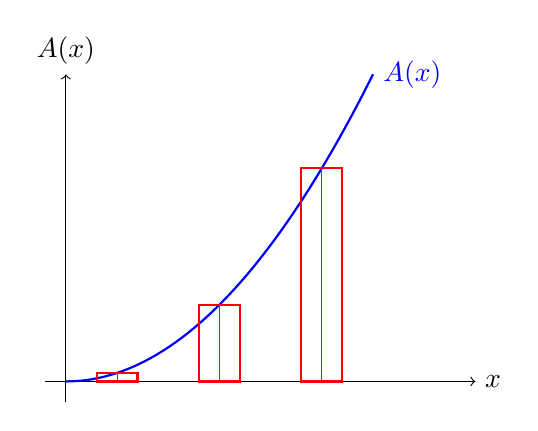
\begin{tikzpicture}[scale=1.3]
\draw[->] (-0.2,0) -- (4,0) node[right] {$x$};
\draw[->] (0,-0.2) -- (0,3) node[above] {$A(x)$};

\draw[domain=0:3, smooth, variable=\x, blue, thick]
  plot ({\x},{(\x)^2/3}) node[right] {$A(x)$};

\foreach \x in {0.5,1.5,2.5}{
  \draw[red] (\x,0) -- (\x,{(\x)^2/3});
  \draw[red, thick] (\x-0.2,0) rectangle (\x+0.2,{(\x)^2/3});
}
\end{tikzpicture}\end{fitbox}
\end{center}
\end{frame}

\section{Эргүүлж үүсгэсэн биет}
\subsection{Дискний арга}
\begin{frame}[allowframebreaks]{Дискний арга}
\[
V=\pi\int_{a}^{b} f(x)^2\,dx.
\]
\end{frame}

\subsection{Бүрхүүл (shell) арга}
\begin{frame}[allowframebreaks]{Бүрхүүл (shell) арга}
\[
V = 2\pi\int_{a}^{b} x f(x)\,dx.
\]
\end{frame}

\subsection*{Жишээ}
\begin{frame}[allowframebreaks]{Жишээ}
$y=\sqrt{x}$ муруйг $y$-тэнхлэгийн эргэн эргүүлэх ($0\le x\le4$):
\[
V=2\pi\int_{0}^{4} x\sqrt{x} dx = \frac{128\pi}{5}.
\]
\end{frame}

\subsection*{TikZ зураг}
\begin{frame}[allowframebreaks]{TikZ зураг}
\begin{center}
\begin{fitbox}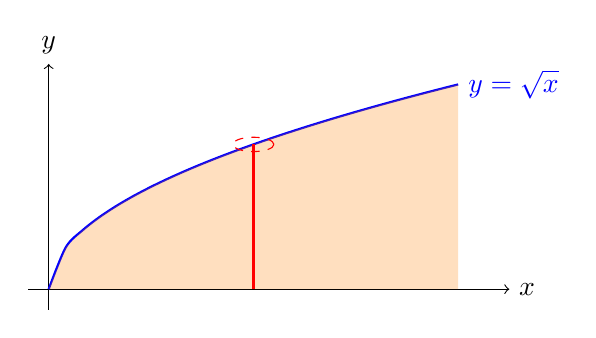
\begin{tikzpicture}[scale=1.3]

\draw[->] (-0.2,0)--(4.5,0) node[right] {$x$};
\draw[->] (0,-0.2)--(0,2.2) node[above] {$y$};

\draw[domain=0:4, smooth, variable=\x, blue, thick]
  plot({\x},{sqrt(\x)}) node[right] {$y=\sqrt{x}$};

\fill[orange, opacity=.25] (0,0)--plot[domain=0:4]({\x},{sqrt(\x)})--(4,0)--cycle;

\draw[red, thick] (2,0)--(2,{sqrt(2)});
\draw[red, dashed] (2,{sqrt(2)}) circle (0.2 and 0.07);

\end{tikzpicture}\end{fitbox}
\end{center}
\end{frame}

\section{Нэмэлт жишээ — 2 муруйн хоорондох талбай}
\begin{frame}[allowframebreaks]{Нэмэлт жишээ — 2 муруйн хоорондох талбай}
$f(x)=\cos x$, $g(x)=\sin x$, $[0,\pi/4]$ интервал дахь талбай:

\[
A=\int_{0}^{\pi/4} (\cos x - \sin x)\, dx.
\]
\end{frame}

% Семинар ба гэрийн даалгавар (Берманы бодлогын хураамжаас)
% Лекц 16: семинар ба гэрийн даалгавар. Бодлогууд: Г.Н. Берман, "Сборник задач по курсу
% математического анализа" (22-р хэвлэл). [Б.N] нь номын бодлогын дугаар.

\ProblemSet{Семинар 16}
\begin{frame}[allowframebreaks]{Семинар 16}
\pgroup{Хязгааргүй хилтэй өргөтгөсөн интегралыг бод (эсвэл сарнихыг тогтоо).}
\begin{plist}
\prob{2366}{$\int_1^{+\infty}\frac{dx}{x^4}$}
\prob{2367}{$\int_1^{+\infty}\frac{dx}{\sqrt x}$}
\prob{2368}{$\int_0^{+\infty}e^{-ax}dx$ \ ($a>0$)}
\prob{2369}{$\int_{-\infty}^{+\infty}\frac{2x\,dx}{x^2+1}$}
\prob{2370}{$\int_{-\infty}^{+\infty}\frac{dx}{x^2+2x+2}$}
\prob{2376}{$\int_0^{+\infty}xe^{-x^2}dx$}
\prob{2380}{$\int_0^{+\infty}e^{-x}\sin x\,dx$}
\end{plist}
\pgroup{Нийлэлтийг шинжил.}
\begin{plist}
\prob{2386}{$\int_0^{+\infty}\frac{x\,dx}{x^3+1}$}
\prob{2387}{$\int_1^{+\infty}\frac{x^3+1}{x^4}\,dx$}
\prob{2412}{$\int_0^1\frac{\sqrt x\,dx}{\sqrt{1-x^4}}$}
\end{plist}
\pgroup{Үл зааглагдах функцийн интегралыг бод (эсвэл сарнихыг тогтоо).}
\begin{plist}
\prob{2394}{$\int_0^1\frac{dx}{\sqrt{1-x^2}}$}
\prob{2395}{$\int_0^2\frac{dx}{x^2-4x+3}$}
\prob{2397}{$\int_0^1x\ln x\,dx$}
\prob{2399}{$\int_1^2\frac{dx}{x\ln x}$}
\end{plist}
\pgroup{Талбай ба эзлэхүүн.}
\begin{plist}
\prob{1600}{$y=x^2-6x+10$ ба $y=6x-x^2$ параболуудаар хүрээлэгдсэн дүрсийн талбайг ол.}
\prob{2460}{$y=x^2$ ба $y=\frac{x^3}{3}$ шугамуудаар хүрээлэгдсэн дүрсийн талбайг ол.}
\prob{2478}{$y=e^x$, $y=e^{-x}$ ба $x=1$ шулуунаар хүрээлэгдсэн дүрсийн талбайг ол.}
\prob{2559}{$y=xe^x$, $x=1$, $y=0$ шугамуудаар хүрээлэгдсэн муруй шугаман трапецийг $Ox$ тэнхлэгийг тойруулан эргүүлэхэд үүсэх биетийн эзлэхүүнийг ол.}
\prob{2561}{$y=x^2$ ба $y^2=x$ параболуудаар хүрээлэгдсэн дүрсийг $Ox$ тэнхлэгийг тойруулан эргүүлэхэд үүсэх биетийн эзлэхүүнийг ол.}
\prob{2564}{$y=2x-x^2$ парабол ба $Ox$ тэнхлэгээр хүрээлэгдсэн дүрсийг $Oy$ тэнхлэгийг тойруулан эргүүлэхэд үүсэх биетийн эзлэхүүнийг ол.}
\end{plist}
\end{frame}

\ProblemSet{Гэрийн даалгавар 16}
\begin{frame}[allowframebreaks]{Гэрийн даалгавар 16}
\pgroup{Хязгааргүй хилтэй өргөтгөсөн интегралыг бод (эсвэл сарнихыг тогтоо).}
\begin{plist}
\prob{2371}{$\int_2^{+\infty}\frac{\ln x}{x}\,dx$}
\prob{2372}{$\int_1^{+\infty}\frac{dx}{x^2(x+1)}$}
\prob{2373}{$\int_0^{+\infty}\frac{x\,dx}{(1+x)^3}$}
\prob{2377}{$\int_0^{+\infty}x^3e^{-x^2}dx$}
\prob{2378}{$\int_0^{+\infty}x\sin x\,dx$}
\prob{2381}{$\int_0^{+\infty}e^{-ax}\cos bx\,dx$ \ ($a>0$)}
\prob{2382}{$\int_1^{+\infty}\frac{\arctg x}{x^2}\,dx$}
\prob{2383}{$\int_0^{+\infty}\frac{dx}{1+x^3}$}
\prob{2385}{$\int_1^{+\infty}\frac{\sqrt x\,dx}{(1+x)^2}$}
\end{plist}
\pgroup{Нийлэлтийг шинжил.}
\begin{plist}
\prob{2389}{$\int_1^{+\infty}\frac{\ln(x^2+1)}{x}\,dx$}
\prob{2390}{$\int_0^{+\infty}\sqrt x\,e^{-x}dx$}
\prob{2392}{$\int_{e^2}^{+\infty}\frac{dx}{x\ln\ln x}$}
\prob{2393}{$\int_e^{+\infty}\frac{dx}{x(\ln x)^{3/2}}$}
\prob{2413}{$\int_0^1\frac{x^2\,dx}{\sqrt[3]{(1-x^2)^5}}$}
\prob{2414}{$\int_0^1\frac{dx}{e^{\sqrt x}-1}$}
\end{plist}
\pgroup{Үл зааглагдах функцийн интегралыг бод (эсвэл сарнихыг тогтоо).}
\begin{plist}
\prob{2398}{$\int_0^{1/e}\frac{dx}{x\ln^2x}$}
\prob{2400}{$\int_1^e\frac{dx}{x\sqrt{\ln x}}$}
\prob{2402}{$\int_a^b\frac{x\,dx}{\sqrt{(x-a)(b-x)}}$ \ ($a<b$)}
\prob{2405}{$\int_{-1}^1\frac{dx}{(2-x)\sqrt{1-x^2}}$}
\prob{2406}{$\int_{-1}^1\frac{3x^2+2}{\sqrt[3]{x^2}}\,dx$}
\prob{2411}{$\int_0^1\frac{e^{1/x}}{x^3}\,dx$}
\end{plist}
\pgroup{Талбай.}
\begin{plist}
\prob{1601}{$y=x^2-2x+2$ парабол, түүний $(3,5)$ цэг дээрх шүргэгч, $Oy$ ба $Ox$ тэнхлэгүүдээр хүрээлэгдсэн дүрсийн талбайг ол.}
\prob{2459}{$y^2+8x=16$ ба $y^2-24x=48$ параболуудаар хүрээлэгдсэн дүрсийн талбайг ол.}
\prob{2468}{$y=x(x-1)^2$ шугам ба абсциссын тэнхлэгээр хүрээлэгдсэн дүрсийн талбайг ол.}
\prob{2483}{$y=\ln x$ ба $y=\ln^2x$ шугамуудаар хүрээлэгдсэн дүрсийн талбайг ол.}
\prob{2485}{Абсциссын тэнхлэг, $y=\sin x$ ба $y=\cos x$ шугамуудаар хүрээлэгдсэн муруй шугаман гурвалжнуудын нэгийн талбайг ол.}
\end{plist}
\pgroup{Эзлэхүүн.}
\begin{plist}
\prob{2555}{$y^2=4x$ параболыг тэнхлэгийг нь тойруулан эргүүлэхэд үүсэх гадаргуу ба оройгоос 1 нэгжийн зайд, тэнхлэгт перпендикуляр хавтгайгаар хүрээлэгдсэн биетийн эзлэхүүнийг ол.}
\prob{2556}{Их тэнхлэг нь $2a$, бага тэнхлэг нь $2b$ эллипсийг 1) их тэнхлэгийг нь, 2) бага тэнхлэгийг нь тойруулан эргүүлэв. Үүсэх эллипсоидуудын эзлэхүүнийг ол. Тухайн тохиолдолд бөмбөрцгийн эзлэхүүнийг гарга.}
\prob{2563}{$y=\arcsin x$ шугамаар хүрээлэгдсэн, $[0,1]$ суурьтай муруй шугаман трапецийг $Ox$ тойруулан эргүүлэхэд үүсэх биетийн эзлэхүүнийг ол.}
\prob{2565}{$y=\sin x$ синусоидын хагас үеийн нумаар хүрээлэгдсэн муруй шугаман трапецийг $Oy$ тэнхлэгийг тойруулан эргүүлэхэд үүсэх биетийн эзлэхүүнийг ол.}
\end{plist}
\end{frame}

